% GNUPLOT: LaTeX picture with Postscript
\begingroup
  \makeatletter
  \providecommand\color[2][]{%
    \GenericError{(gnuplot) \space\space\space\@spaces}{%
      Package color not loaded in conjunction with
      terminal option `colourtext'%
    }{See the gnuplot documentation for explanation.%
    }{Either use 'blacktext' in gnuplot or load the package
      color.sty in LaTeX.}%
    \renewcommand\color[2][]{}%
  }%
  \providecommand\includegraphics[2][]{%
    \GenericError{(gnuplot) \space\space\space\@spaces}{%
      Package graphicx or graphics not loaded%
    }{See the gnuplot documentation for explanation.%
    }{The gnuplot epslatex terminal needs graphicx.sty or graphics.sty.}%
    \renewcommand\includegraphics[2][]{}%
  }%
  \providecommand\rotatebox[2]{#2}%
  \@ifundefined{ifGPcolor}{%
    \newif\ifGPcolor
    \GPcolortrue
  }{}%
  \@ifundefined{ifGPblacktext}{%
    \newif\ifGPblacktext
    \GPblacktexttrue
  }{}%
  % define a \g@addto@macro without @ in the name:
  \let\gplgaddtomacro\g@addto@macro
  % define empty templates for all commands taking text:
  \gdef\gplbacktext{}%
  \gdef\gplfronttext{}%
  \makeatother
  \ifGPblacktext
    % no textcolor at all
    \def\colorrgb#1{}%
    \def\colorgray#1{}%
  \else
    % gray or color?
    \ifGPcolor
      \def\colorrgb#1{\color[rgb]{#1}}%
      \def\colorgray#1{\color[gray]{#1}}%
      \expandafter\def\csname LTw\endcsname{\color{white}}%
      \expandafter\def\csname LTb\endcsname{\color{black}}%
      \expandafter\def\csname LTa\endcsname{\color{black}}%
      \expandafter\def\csname LT0\endcsname{\color[rgb]{1,0,0}}%
      \expandafter\def\csname LT1\endcsname{\color[rgb]{0,1,0}}%
      \expandafter\def\csname LT2\endcsname{\color[rgb]{0,0,1}}%
      \expandafter\def\csname LT3\endcsname{\color[rgb]{1,0,1}}%
      \expandafter\def\csname LT4\endcsname{\color[rgb]{0,1,1}}%
      \expandafter\def\csname LT5\endcsname{\color[rgb]{1,1,0}}%
      \expandafter\def\csname LT6\endcsname{\color[rgb]{0,0,0}}%
      \expandafter\def\csname LT7\endcsname{\color[rgb]{1,0.3,0}}%
      \expandafter\def\csname LT8\endcsname{\color[rgb]{0.5,0.5,0.5}}%
    \else
      % gray
      \def\colorrgb#1{\color{black}}%
      \def\colorgray#1{\color[gray]{#1}}%
      \expandafter\def\csname LTw\endcsname{\color{white}}%
      \expandafter\def\csname LTb\endcsname{\color{black}}%
      \expandafter\def\csname LTa\endcsname{\color{black}}%
      \expandafter\def\csname LT0\endcsname{\color{black}}%
      \expandafter\def\csname LT1\endcsname{\color{black}}%
      \expandafter\def\csname LT2\endcsname{\color{black}}%
      \expandafter\def\csname LT3\endcsname{\color{black}}%
      \expandafter\def\csname LT4\endcsname{\color{black}}%
      \expandafter\def\csname LT5\endcsname{\color{black}}%
      \expandafter\def\csname LT6\endcsname{\color{black}}%
      \expandafter\def\csname LT7\endcsname{\color{black}}%
      \expandafter\def\csname LT8\endcsname{\color{black}}%
    \fi
  \fi
    \setlength{\unitlength}{0.0500bp}%
    \ifx\gptboxheight\undefined%
      \newlength{\gptboxheight}%
      \newlength{\gptboxwidth}%
      \newsavebox{\gptboxtext}%
    \fi%
    \setlength{\fboxrule}{0.5pt}%
    \setlength{\fboxsep}{1pt}%
    \definecolor{tbcol}{rgb}{1,1,1}%
\begin{picture}(9060.00,7360.00)%
    \gplgaddtomacro\gplbacktext{%
      \csname LTb\endcsname%%
      \put(438,4176){\makebox(0,0)[r]{\strut{}$0$}}%
      \csname LTb\endcsname%%
      \put(438,4512){\makebox(0,0)[r]{\strut{}$2$}}%
      \csname LTb\endcsname%%
      \put(438,4848){\makebox(0,0)[r]{\strut{}$4$}}%
      \csname LTb\endcsname%%
      \put(438,5184){\makebox(0,0)[r]{\strut{}$6$}}%
      \csname LTb\endcsname%%
      \put(438,5520){\makebox(0,0)[r]{\strut{}$8$}}%
      \csname LTb\endcsname%%
      \put(438,5856){\makebox(0,0)[r]{\strut{}$10$}}%
      \csname LTb\endcsname%%
      \put(438,6192){\makebox(0,0)[r]{\strut{}$12$}}%
      \csname LTb\endcsname%%
      \put(438,6528){\makebox(0,0)[r]{\strut{}$14$}}%
      \csname LTb\endcsname%%
      \put(438,6864){\makebox(0,0)[r]{\strut{}$16$}}%
      \csname LTb\endcsname%%
      \put(518,4018){\makebox(0,0){\strut{}0.0$\times10^{0}$}}%
      \csname LTb\endcsname%%
      \put(988,4018){\makebox(0,0){\strut{}2.0$\times10^{5}$}}%
      \csname LTb\endcsname%%
      \put(1459,4018){\makebox(0,0){\strut{}4.0$\times10^{5}$}}%
      \csname LTb\endcsname%%
      \put(1929,4018){\makebox(0,0){\strut{}6.0$\times10^{5}$}}%
      \csname LTb\endcsname%%
      \put(2399,4018){\makebox(0,0){\strut{}8.0$\times10^{5}$}}%
      \csname LTb\endcsname%%
      \put(2869,4018){\makebox(0,0){\strut{}1.0$\times10^{6}$}}%
      \csname LTb\endcsname%%
      \put(3339,4018){\makebox(0,0){\strut{}1.2$\times10^{6}$}}%
      \csname LTb\endcsname%%
      \put(3809,4018){\makebox(0,0){\strut{}1.4$\times10^{6}$}}%
      \csname LTb\endcsname%%
      \put(4279,4018){\makebox(0,0){\strut{}1.6$\times10^{6}$}}%
    }%
    \gplgaddtomacro\gplfronttext{%
      \csname LTb\endcsname%%
      \put(139,5520){\rotatebox{-270.00}{\makebox(0,0){\strut{}Difference from finest mesh (\%)}}}%
      \csname LTb\endcsname%%
      \put(2399,3780){\makebox(0,0){\strut{}Number of volume cells}}%
      \csname LTb\endcsname%%
      \put(2399,7102){\makebox(0,0){\strut{}Resistance (Pa/(L/min))}}%
    }%
    \gplgaddtomacro\gplbacktext{%
      \csname LTb\endcsname%%
      \put(5118,4176){\makebox(0,0)[r]{\strut{}$0$}}%
      \csname LTb\endcsname%%
      \put(5118,4512){\makebox(0,0)[r]{\strut{}$0.05$}}%
      \csname LTb\endcsname%%
      \put(5118,4848){\makebox(0,0)[r]{\strut{}$0.1$}}%
      \csname LTb\endcsname%%
      \put(5118,5184){\makebox(0,0)[r]{\strut{}$0.15$}}%
      \csname LTb\endcsname%%
      \put(5118,5520){\makebox(0,0)[r]{\strut{}$0.2$}}%
      \csname LTb\endcsname%%
      \put(5118,5856){\makebox(0,0)[r]{\strut{}$0.25$}}%
      \csname LTb\endcsname%%
      \put(5118,6192){\makebox(0,0)[r]{\strut{}$0.3$}}%
      \csname LTb\endcsname%%
      \put(5118,6528){\makebox(0,0)[r]{\strut{}$0.35$}}%
      \csname LTb\endcsname%%
      \put(5118,6864){\makebox(0,0)[r]{\strut{}$0.4$}}%
      \csname LTb\endcsname%%
      \put(5199,4018){\makebox(0,0){\strut{}0.0$\times10^{0}$}}%
      \csname LTb\endcsname%%
      \put(5649,4018){\makebox(0,0){\strut{}2.0$\times10^{5}$}}%
      \csname LTb\endcsname%%
      \put(6099,4018){\makebox(0,0){\strut{}4.0$\times10^{5}$}}%
      \csname LTb\endcsname%%
      \put(6549,4018){\makebox(0,0){\strut{}6.0$\times10^{5}$}}%
      \csname LTb\endcsname%%
      \put(6999,4018){\makebox(0,0){\strut{}8.0$\times10^{5}$}}%
      \csname LTb\endcsname%%
      \put(7449,4018){\makebox(0,0){\strut{}1.0$\times10^{6}$}}%
      \csname LTb\endcsname%%
      \put(7899,4018){\makebox(0,0){\strut{}1.2$\times10^{6}$}}%
      \csname LTb\endcsname%%
      \put(8349,4018){\makebox(0,0){\strut{}1.4$\times10^{6}$}}%
      \csname LTb\endcsname%%
      \put(8799,4018){\makebox(0,0){\strut{}1.6$\times10^{6}$}}%
    }%
    \gplgaddtomacro\gplfronttext{%
      \csname LTb\endcsname%%
      \put(4659,5520){\rotatebox{-270.00}{\makebox(0,0){\strut{}Difference from finest mesh (\%)}}}%
      \csname LTb\endcsname%%
      \put(6999,3780){\makebox(0,0){\strut{}Number of volume cells}}%
      \csname LTb\endcsname%%
      \put(6999,7102){\makebox(0,0){\strut{}Right-lung flow fraction (\%)}}%
    }%
    \gplgaddtomacro\gplbacktext{%
      \csname LTb\endcsname%%
      \put(358,506){\makebox(0,0)[r]{\strut{}$0$}}%
      \csname LTb\endcsname%%
      \put(358,890){\makebox(0,0)[r]{\strut{}$1$}}%
      \csname LTb\endcsname%%
      \put(358,1274){\makebox(0,0)[r]{\strut{}$2$}}%
      \csname LTb\endcsname%%
      \put(358,1658){\makebox(0,0)[r]{\strut{}$3$}}%
      \csname LTb\endcsname%%
      \put(358,2042){\makebox(0,0)[r]{\strut{}$4$}}%
      \csname LTb\endcsname%%
      \put(358,2426){\makebox(0,0)[r]{\strut{}$5$}}%
      \csname LTb\endcsname%%
      \put(358,2810){\makebox(0,0)[r]{\strut{}$6$}}%
      \csname LTb\endcsname%%
      \put(358,3194){\makebox(0,0)[r]{\strut{}$7$}}%
      \csname LTb\endcsname%%
      \put(438,348){\makebox(0,0){\strut{}0.0$\times10^{0}$}}%
      \csname LTb\endcsname%%
      \put(918,348){\makebox(0,0){\strut{}2.0$\times10^{5}$}}%
      \csname LTb\endcsname%%
      \put(1398,348){\makebox(0,0){\strut{}4.0$\times10^{5}$}}%
      \csname LTb\endcsname%%
      \put(1879,348){\makebox(0,0){\strut{}6.0$\times10^{5}$}}%
      \csname LTb\endcsname%%
      \put(2359,348){\makebox(0,0){\strut{}8.0$\times10^{5}$}}%
      \csname LTb\endcsname%%
      \put(2839,348){\makebox(0,0){\strut{}1.0$\times10^{6}$}}%
      \csname LTb\endcsname%%
      \put(3319,348){\makebox(0,0){\strut{}1.2$\times10^{6}$}}%
      \csname LTb\endcsname%%
      \put(3799,348){\makebox(0,0){\strut{}1.4$\times10^{6}$}}%
      \csname LTb\endcsname%%
      \put(4279,348){\makebox(0,0){\strut{}1.6$\times10^{6}$}}%
    }%
    \gplgaddtomacro\gplfronttext{%
      \csname LTb\endcsname%%
      \put(139,1850){\rotatebox{-270.00}{\makebox(0,0){\strut{}Difference from finest mesh (\%)}}}%
      \csname LTb\endcsname%%
      \put(2359,110){\makebox(0,0){\strut{}Number of volume cells}}%
      \csname LTb\endcsname%%
      \put(2359,3432){\makebox(0,0){\strut{}Right-superior share of right flow (\%)}}%
    }%
    \gplgaddtomacro\gplbacktext{%
      \csname LTb\endcsname%%
      \put(5038,506){\makebox(0,0)[r]{\strut{}$0$}}%
      \csname LTb\endcsname%%
      \put(5038,842){\makebox(0,0)[r]{\strut{}$0.5$}}%
      \csname LTb\endcsname%%
      \put(5038,1178){\makebox(0,0)[r]{\strut{}$1$}}%
      \csname LTb\endcsname%%
      \put(5038,1514){\makebox(0,0)[r]{\strut{}$1.5$}}%
      \csname LTb\endcsname%%
      \put(5038,1850){\makebox(0,0)[r]{\strut{}$2$}}%
      \csname LTb\endcsname%%
      \put(5038,2186){\makebox(0,0)[r]{\strut{}$2.5$}}%
      \csname LTb\endcsname%%
      \put(5038,2522){\makebox(0,0)[r]{\strut{}$3$}}%
      \csname LTb\endcsname%%
      \put(5038,2858){\makebox(0,0)[r]{\strut{}$3.5$}}%
      \csname LTb\endcsname%%
      \put(5038,3194){\makebox(0,0)[r]{\strut{}$4$}}%
      \csname LTb\endcsname%%
      \put(5118,348){\makebox(0,0){\strut{}0.0$\times10^{0}$}}%
      \csname LTb\endcsname%%
      \put(5579,348){\makebox(0,0){\strut{}2.0$\times10^{5}$}}%
      \csname LTb\endcsname%%
      \put(6039,348){\makebox(0,0){\strut{}4.0$\times10^{5}$}}%
      \csname LTb\endcsname%%
      \put(6499,348){\makebox(0,0){\strut{}6.0$\times10^{5}$}}%
      \csname LTb\endcsname%%
      \put(6959,348){\makebox(0,0){\strut{}8.0$\times10^{5}$}}%
      \csname LTb\endcsname%%
      \put(7419,348){\makebox(0,0){\strut{}1.0$\times10^{6}$}}%
      \csname LTb\endcsname%%
      \put(7879,348){\makebox(0,0){\strut{}1.2$\times10^{6}$}}%
      \csname LTb\endcsname%%
      \put(8339,348){\makebox(0,0){\strut{}1.4$\times10^{6}$}}%
      \csname LTb\endcsname%%
      \put(8799,348){\makebox(0,0){\strut{}1.6$\times10^{6}$}}%
    }%
    \gplgaddtomacro\gplfronttext{%
      \csname LTb\endcsname%%
      \put(4659,1850){\rotatebox{-270.00}{\makebox(0,0){\strut{}Difference from finest mesh (\%)}}}%
      \csname LTb\endcsname%%
      \put(6959,110){\makebox(0,0){\strut{}Number of volume cells}}%
      \csname LTb\endcsname%%
      \put(6959,3432){\makebox(0,0){\strut{}Matched-section peak velocity (m/s)}}%
    }%
    \gplbacktext
    \put(0,0){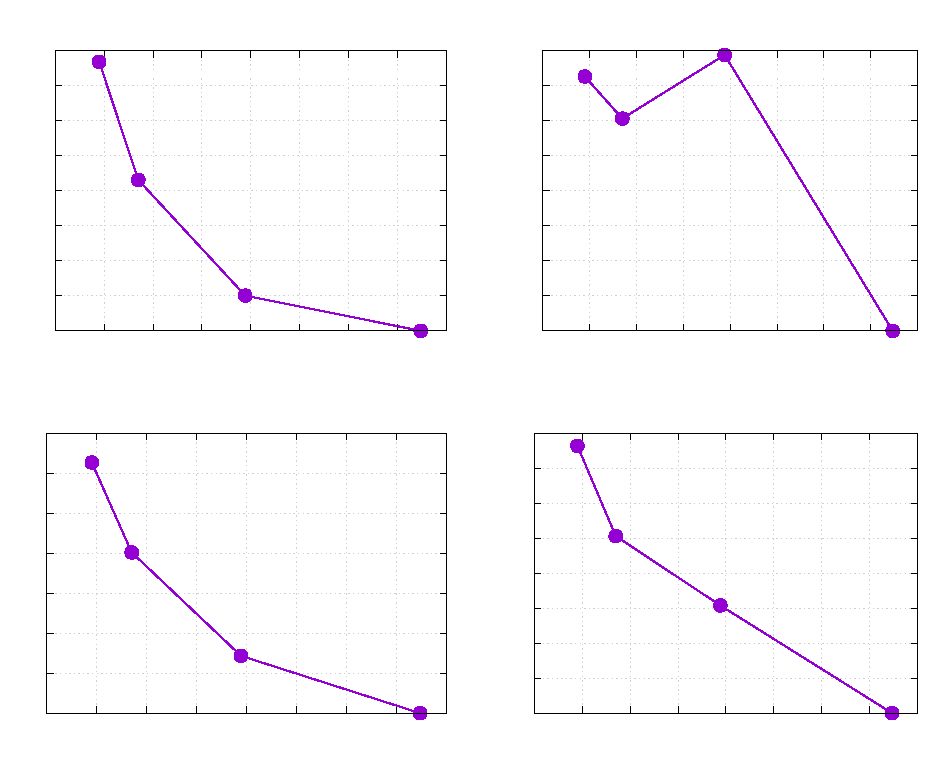
\includegraphics[width={453.00bp},height={368.00bp}]{figures/assignment5_mesh_differences}}%
    \gplfronttext
  \end{picture}%
\endgroup
